\section{Solution}
\label{sec:solution}
\subsection{Training}
The main problem is non-convex and very difficult to optimize. 
One typical solution is to use cyclic coordinate method (CCM)\cite{GorskiPK07}. 
To be specific, we iteratively optimize the objective function by fixing $\mathbf{S}$ with respect to $\mathbf{\Theta}$ and vice versa. 
The major problem in such approach is that the quality of the solution depends highly on the initialization as it converges to a local minimum. 
To be specific, if we get a good estimation of $\mathbf{S}$, it is relatively easy to get a good solution for $\mathbf{\Theta}$ as the final loss function puts more emphasis on the correct region pair matching and vice versa. 

Thus, we propose a region based joint model on saliency estimation and region matching for training. Our pipeline is composed of five main steps: 

1.	\emph{Image level (weak) label generation.} 
In this step, we generate the weak labels based on GPS information automatically. 
Google Map provides satellite images, as well as street view images, together with their GPS information to users, so that we can download them conveniently as database. 
Figure~\ref{fig:dbregion} (color masked) shows the region that our database for Boston dataset (introduced in Section~\ref{sec:expr}) covers. 
The colored masks are drawn by Google Map automatically, indicating the buildings. 
\begin{figure}[t]
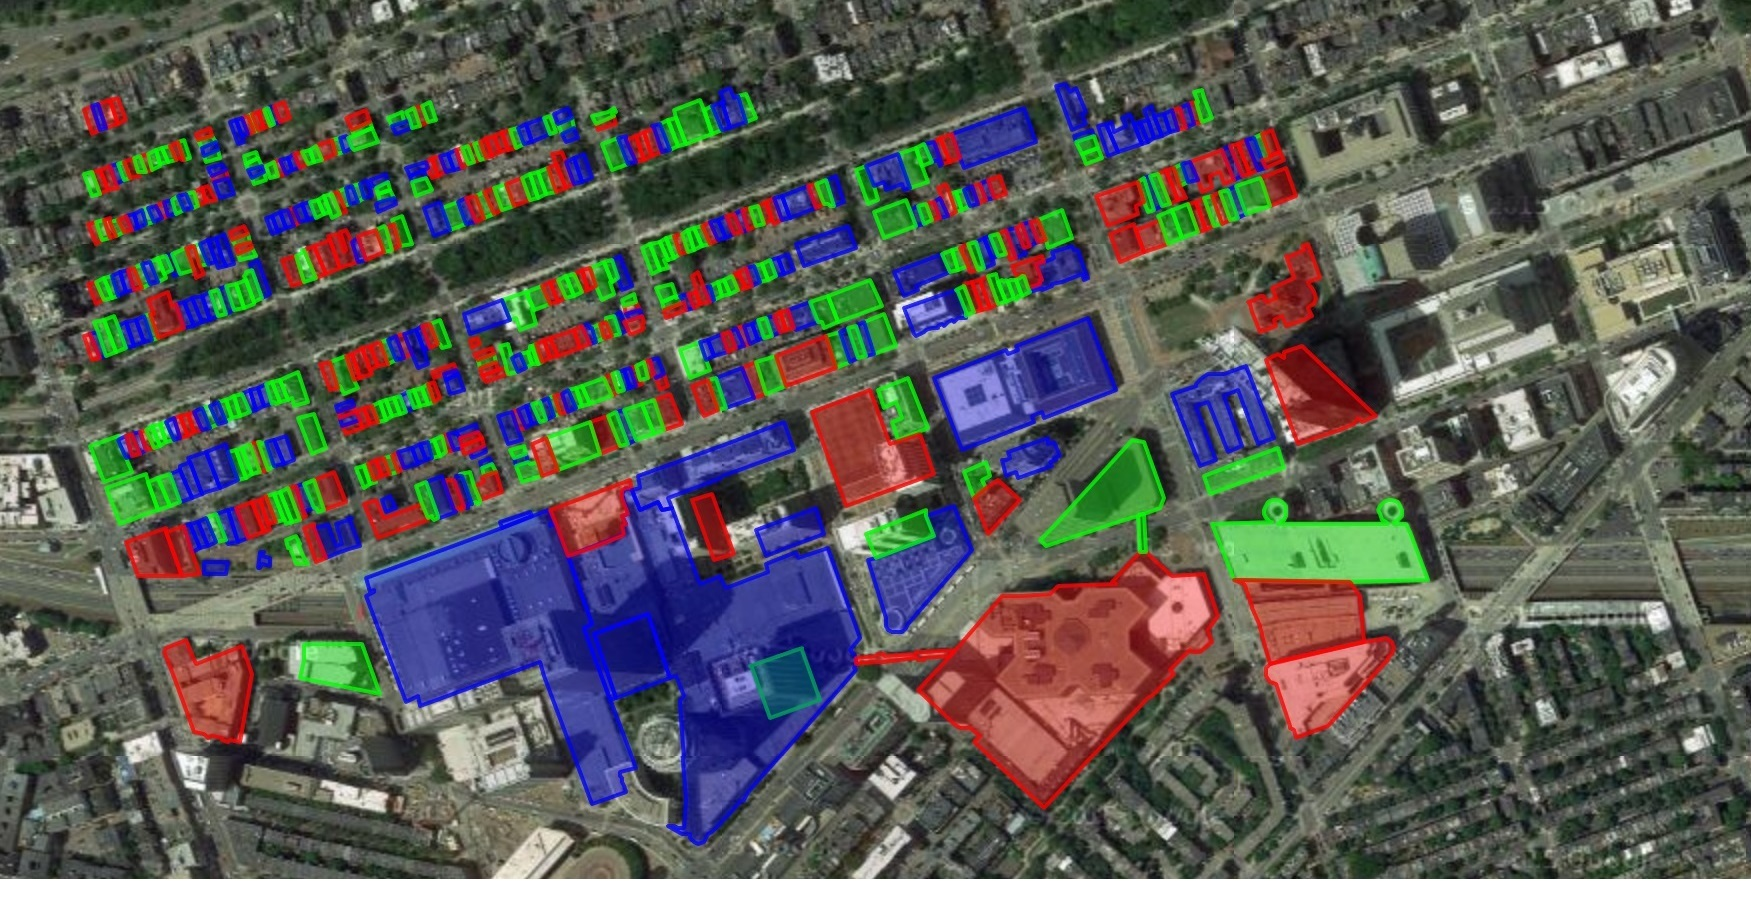
\includegraphics[width=0.7\linewidth]{img/db_region}
\caption{An example for collecting training data with Google Map.}
\label{fig:dbregion}
\end{figure}
After the generation of our database, we sample images in the range that the database covers randomly. 
Google Map provides four different perspectives of view from each point. 
If we just move the sampling point a little, the image with the same perspective would not change a lot. 
Thus, we can get two different images containing almost the same scene, and that is the rationality of our method to generate weak labels automatically.
More specifically, we use Euclidean distance to judge whether two sampling points are near to each other. 
We set the matching label of two images $q, d$ using 
\begin{equation}
\label{eq:weaklabel}
y_{(q, d)} = \left\{
\begin{aligned}
1 \qquad & dist(q,d) \leq \theta \\
0 \qquad & dist(q,d) > \theta
\end{aligned}
\right.
\end{equation}
where $q$ is the sampled image, $d$ is the image from our database, $dist(q,d)$ is the Euclidean distance between the locations of $q$ and $d$ in the real world, $\theta$ is a hyper-parameter that denotes the distance threshold of matching. 
In addition, by zooming, rotating and shifting, we can augment our database to let it contain images with larger diversity. 
Thus, we have completed the generation of training data $D_{train}$.
For database generation, we set $\theta = 25m$.\\[-0.25cm]

2. \emph{Initialization of matching model.}
In this step, we choose a good initialization of matching model. 
To be specific, we train a matching model $m(q_i, d_j; \mathbf{\Theta})$ directly using the image pairs. 
The structure of the network should be the same as that in the following procedure.
That is, we start from the degenerate case where the entire image is treated as one region.

In our training procedure, we applied Siamese network for initializing the matching model. 
The structure of the Siamese network we applied is shown in Figure~\ref{fig:siamese}.
The CNN is used to extract features from images. 
In this step, the region pairs are exactly image pairs themselves. 
We will introduce more details about the structure of the network in \emph{Step 4}.
\begin{figure}[htbp]
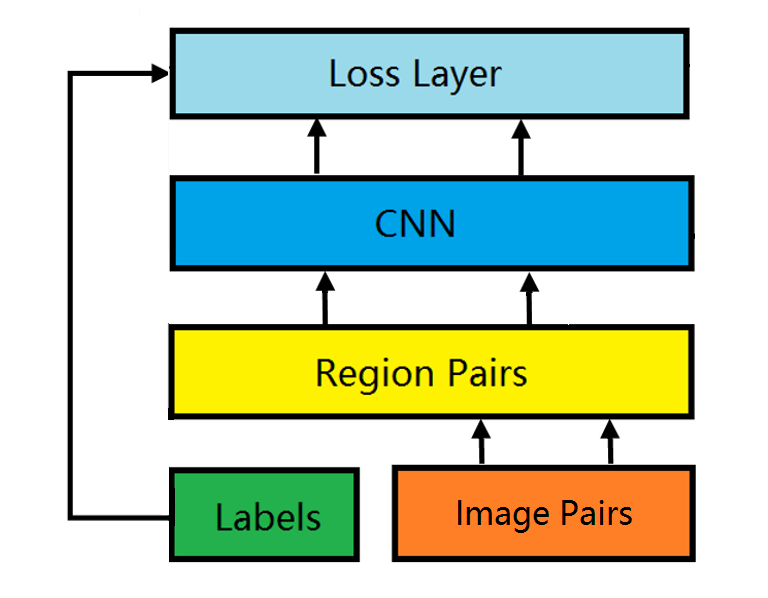
\includegraphics[width=0.6\linewidth]{img/siamese}
\caption{The structure of Siamese network. }
\label{fig:siamese}
\end{figure}

3. \emph{Saliency Estimation}. Apply the matching model $m(q_i, d_j; \mathbf{\Theta})$ on regions and optimize the main problem with respect to saliency $\mathbf{S}$. This problem can be decomposed to $|Q|+|D|$ separate linear objective quadratic constraint convex optimization problems:
\begin{equation}
\label{eq:decomposed_problem}
\begin{aligned}
& \max_{\mathbf{s}(q)} \sum_{q_i \in q} (m_{i\cdot}^+ - m_{i\cdot}^-) s(q_i) \\
\text{where} \\
m_{i\cdot}^+& = \sum_{\{d_j|y(q_i,d_j)=1\}} m(q_i,d_j) \\
m_{i\cdot}^-&=\sum_{\{d_j|y(q_i,d_j)=0\}} \min(0, m(q_i,d_j)-\Delta^{'})\\
s.t.& ||\mathbf{s}(q)||_2 = 1\\
& s(q_i)\in [0,1]
\end{aligned}
\end{equation}
We can add the other $|D|$ formulas with respect to $d$ analogously.
This problem has closed form solution:
\begin{equation}
\label{eq:closed_form_solution}
\begin{aligned}
& \mathbf{m}_q = [..., m_{i\cdot }^+ - m_{i\cdot}^-, ...] \geq \mathbf{0} \\
& \hat{\mathbf{s}}(q) = \frac{\mathbf{m}_q}{||\mathbf{m_q}||_2}
\end{aligned}
\end{equation}
Here, $m_{i\cdot }^+, m_{i\cdot}^-$ correspond to the matching status of $q_i$ to regions in positive labels and those in negative labels. 
Note that $m(q_i, d_j)$ is always non-negative due to our constraint in the section of problem formulation, $m_{i\cdot }^+$ is always non-negative and $m_{i\cdot }^-$ is always non-positive. Hence, we have the solution vector  $ \mathbf{m}_q = [..., m_{i\cdot }^+ - m_{i\cdot}^-, ...] \geq \mathbf{0} $. Analogously, we can compute the solution for $\hat{\mathbf{s}}(d)$.

The solution saliency $\hat{\mathbf{S}} = \{\hat{\mathbf{s}}(q)\} \cup \{\hat{\mathbf{s}}(d)\}$ can be used to generate pseudo labels on region level. 
The label is called ``pseudo'' because we fix the parameter $\mathbf{\Theta}$ from an imperfect matching model $m(q_i, d_j; \mathbf{\Theta})$ to get the solution. 

With the hypothesis that different parts of a building would not look very different, if an image pair $(q,d)$ is labelled as matched, then the pair of salient regions $(q_i, d_j)$ with high $s(q_i)$ and $s(d_j)$ should be matched with high level confidence. 
Oppositely,  if an image pair $(q,d)$ is labelled as unmatched, the pair of salient regions $(q_i, d_j)$ with high $s(q_i)$ and $s(d_j)$ should be unmatched with high level confidence, too. 
Thus, we use Eq~\eqref{eq:weight} (i.e. the sum of $s(q_i)$ and $s(d_j)$) to measure the confidence of the pseudo label $y_{(q,d)}$ for region pair $(q_i, d_j)$.

4. \emph{Region based matching optimization}. After estimating the saliency score of each region, we only use most confident pseudo region level labels to train the region matching model $m(q_i, d_j; \mathbf{\Theta})$. 
To refine the region level matching model, we minimize Eq~\eqref{eq:region_loss} as the loss function with the Siamese network structure, which has been shown in Figure~\ref{fig:siamese}. 
Since the training samples are fed to the network one by one (or batch by batch), the loss function for a region pair $(q_i, d_j)$ with label $y$ should be rewritten as 
\begin{equation}
L(q_i, d_j, y) = y\cdot m(q_i, d_j) + (1-y)\cdot \max(0, \Delta^{'} - m(q_i,d_j))
\label{eq:region_loss_sum}
\end{equation} 
where $\Delta^{'}$ is the hyper-parameter to keep unmatched pairs having a small matching score. 

5. We repeat step 3 and step 4 and gradually lower the confidence level for the pseudo label as the model becomes more and more accurate and we could rely on more pseudo labels generated. 
The confidence lowering procedure is controlled by the self-paced function\cite{jiang2015self}. 

In self-paced curriculum learning, a the self-paced function $f(\mathbf{v};\lambda)$ determines a learning scheme, where $\mathbf{v}\in [0,1]^n$ denotes a vector of weight variable for each training sample and $\lambda$ controls the learning pace. 
In a self-paced function, $||\mathbf{v}||_1$ increases with respect to $\lambda$. For a fixed function $f(\mathbf{v};\lambda)$, the sample selecting weight $\mathbf{v}$ can be computed by
\begin{equation}
\mathbf{v} = \argmin_{\mathbf{v}\in [0,1]^n}\sum v_il_i + f(\mathbf{v};\lambda)
\end{equation}
where $l_i$ is the loss function for the $i^{th}$ sample. 

To be more specific, we select training samples $\{(q_i, d_j, y)\}$by 
\begin{equation}
\mathbf{v} = \argmin_{\mathbf{v}\in [0,1]^n}\sum v_{ij}\frac{1}{s(q_i) + s(d_j)} + f(\mathbf{v};\lambda)
\label{eq:sample_selection}
\end{equation}
where $n$ denotes the total number of our candidate samples $(q_i, d_j, y)$. To make the loss function $l_i$ satisfy the requirements of self-paced learning scheme~\cite{jiang2015self}, we set $l_i = \frac{1}{s(q_i) + s(d_j)} $, which is the multiplicative inverse of Eq~\eqref{eq:weight}.

The self-paced function we apply is 
\begin{equation}
f(\mathbf{v};\lambda) = \lambda-||\mathbf{v}||_1 = -\lambda\sum_{i=1}^n v_i
\end{equation}
representing a linear scheme. 

Thus, we reformulate \emph{main problem} into a self-paced version. 

\text{self-paced version of main problem:}
\begin{equation*}
\begin{aligned}
min_{\mathbf{S}, \mathbf{\Theta}} L(q, d, y; \mathbf{S}, \mathbf{\Theta}) &= -y\, \sum_{i, j}\sum_{y_{(q, d)}=1} w_{ij}\, m(q_i, d_j; \mathbf{\Theta}) \\
& - (1-y)\, \sum_{i, j}\sum_{y_{(q, d)}=0} w_{ij}\, \max(\Delta^{'}-m(q_i, d_j; \mathbf{\Theta}))\\
& + f(w_{ij}; \lambda) \\
w_{ij} &= s(q_i) + s(d_j)\\
\mathbf{S} &= \{s(q_i)\} \cup \{s(d_j)\}\\  
f(w_{ij}; \lambda) &= \lambda - ||w_{ij}||_1 \\
s.t. & ||s(q)||_2 = 1 \quad \forall q\\
& ||s(d)||_2 = 1 \quad \forall d\\
& s(q_i), s(d_j) \in [0,1] \\
& y\in \{+1, 0\}
\end{aligned}
\end{equation*}
where $\lambda$ is a hyper-parameter to control the pace of learning in the self-paced procedure. 

In summary, our method can be described as Algorithm~\ref{alg:solution}.
\begin{algorithm}
\begin{algorithmic}[1]  
\REQUIRE{training dataset $D_{train}$, pre-trained matching model parameters $\mathbf{\Theta}$, self-paced function $f$ and stepsize $\mu$}\\
\ENSURE{saliency score $\mathbf{S}$ and refined matching parameters $\mathbf{\Theta^*}$ \\}
~\\
\STATE{Initialize $\mathbf{S}$, $\lambda$ and the matching model $\mathbf{\Theta^* = \Theta}$}
\WHILE{{\sl not converged}}
  \STATE{Estimate saliency score with Eq~\eqref{eq:closed_form_solution}}
  \STATE{Generate region level pseudo labels using image level labels}
  \STATE{Select ``easy'' samples by Eq~\eqref{eq:sample_selection}}
  \STATE{Refine $\mathbf{\Theta^*}$ with the loss function Eq~\eqref{eq:region_loss_sum}}
  \STATE{\textbf{if} $\lambda$ is small \textbf{then} increase $\lambda$ by $\mu$}
\ENDWHILE
\STATE{\textbf{return} $\mathbf{S}$, $\mathbf{\Theta^*}$}
\end{algorithmic}
\caption{Joint Saliency Estimation and Matching Optimization}
\label{alg:solution}
\end{algorithm}

\subsection{Inference}
After refining the matching model, we propose a corresponding region-based metric to measure the similarity between two images $q$ and $d$, which is 
\begin{equation}
sim_R(q,d) = -\sum_{q_i \in q} \min_{d_j\in d} \frac{|q_i|}{|q|} w_{ij}||f(q_i)-f(d_j)||_2
\label{eq:simR}
\end{equation}
where $|q_i|$ and $|q|$ is the size of region $q_i$ and image $q$, $f(q)$ and $f(d)$ are the vector representations of the two images in the feature space. 

Our method of video geo-localization is based on such fact: if a video has not been edited, the geo-location of it should not vary a lot in a short time. 
To find the geo-location of a video, we first retrieve $K$ most similar images in the database for each frame, and collect $K\times F$ images (may overlap) in the database. 
Then, we cluster the images in the database into $C$ clusters, based on their representative vectors in the feature space. 
The video will be localized to the average GPS coordinate of the largest cluster.
